\documentclass[journal]{IEEEtran}
\usepackage{blindtext}
\let\labelindent\relax
\usepackage[inline]{enumitem}
\usepackage{graphicx}
\usepackage[acronym,toc,shortcuts]{glossaries}
\usepackage{subcaption}
\usepackage{float}

% Abstand nach einer Abbildung verringern
\setlength{\belowcaptionskip}{-5pt}


\usepackage{url}
\usepackage{breakurl}
\def\UrlBreaks{\do\/\do-}

\usepackage[bookmarksopen, bookmarksdepth=2, breaklinks=true]{hyperref}
\usepackage[official]{eurosym}
\usepackage{listings}
\usepackage{multicol}
\usepackage[utf8]{inputenc}  
\usepackage[german]{babel}\usepackage{csquotes}
\usepackage[style=ieee, sorting=none, isbn=true, url=true]{biblatex}
\addbibresource{bibtex.bib}

% *** GRAPHICS RELATED PACKAGES ***
%
\ifCLASSINFOpdf
\else
\fi

\newacronym{iaas}{IaaS}{Infrastructure as a Service}
\newacronym{api}{API}{Application Programming Interface}
\newacronym{stt}{STT}{Speech to Text}
\newacronym{tts}{TTS}{Text to Speech}
\newacronym{nlu}{NLU}{Natural Language Unterstanding}
\newacronym{nlc}{NLC}{Natural Language Classification}
\newacronym{sdk}{SDK}{Software Development Kit}
\newacronym{cmu}{CMU}{Carnegie Mellon University}
\newacronym{iso}{ISO}{Disk Image Optical}
\newacronym{aws}{AWS}{Amazon Web Services}
\newacronym{ki}{KI}{künstlichen Intelligenz}

\hyphenation{op-tical net-works semi-conduc-tor}

\begin{document}
\title{Speech Triggered Mobility Support And Privacy}

\author{
\begin{center}
  \begin{tabular}{c c c} 
  Jenni Belov & Marius Becherer & Max Wannenmacher \\ 
  Hochschule Furtwangen &  Hochschule Furtwangen &  Hochschule Furtwangen \\ 
  Jenni.Belov@hs-furtwangen.de & Marius.Becherer@hs-furtwangen.de & Max.Wannenmacher@hs-furtwangen.de \\
  \\
  & Michael Zipperle \\ 
  & Hochschule Furtwangen \\ 
  & Michael.Zipperle@hs-furtwangen.de \\
  \end{tabular}
\end{center}}%
       
%\thanks{M. Shell is with the Department
%of Electrical and Computer Engineering, Georgia Institute of Technology, Atlanta,
%GA, 30332 USA e-mail: (see http://www.michaelshell.org/contact.html).}% <-this % stops a space
%\thanks{J. Doe and J. Doe are with Anonymous University.}% <-this % stops a space
%\thanks{Manuscript received April 19, 2005; revised January 11, 2007.}}

% The paper headers
\markboth{Hochschule Furtwangen - Semesterprojekt, Februar 2019}%
{Hochschule Furtwangen - Semesterprojekt, Februar 2019}

% make the title area
\maketitle

% Note that keywords are not normally used for peerreview papers.
%\begin{IEEEkeywords}
%IEEEtran, journal, \LaTeX, paper, template.
%\end{IEEEkeywords}

% For peerreview papers, this IEEEtran command inserts a page break and
% creates the second title. It will be ignored for other modes.
\IEEEpeerreviewmaketitle


% *** START OF SECTIONS ***--------------------------------------------
\begin{abstract}
%\boldmath 
Aktuelle Sprachassistenten werden von großen IT-Konzernen wie Google, Amazon, Microsoft, Apple oder Baidu angeboten. Die Sprachassistenten umfassen zahlreiche Funktionalitäten, welche i. d. R. zentral in der Cloud von den Anbietern ausgeführt werden. Doch was passiert mit den Eingabedaten der Nutzer? Die Anbieter machen dazu ungenaue Angaben. Die Nutzer können sich nicht sicher sein, ob ihre Privatsphäre und Daten geschützt sind. Es stellt sich die zentrale Forschungsfrage, was mit der sprachbasierten Interaktion zwischen Nutzern und Diensten aktuell geschieht, und welche Konzepte für einen konfigurierbaren Datenschutz durch die Nutzer zukünftig vorstellbar sind. Im Artikel werden die Umfrageergebnisse vorgestellt, die von Sprachassistent-Nutzern im Rahmen dieser Forschungsarbeit ermittelt wurden. Das Ergebnis zeigt insbesondere die Zahlungsbereitschaft für einen individuell konfigurierbaren Datenschutz. Basierend auf den Erkenntnissen der ersten Veröffentlichung dieses Artikels, wird das Konzept für einen konfigurierbaren Sprachassistenten erweitert und prototypisch umgesetzt. Für den Prototyp wird eine konkrete Technologieauswahl getroffen. Anschließend wird der Artikel mit einer Bewertung des Prototyps abgerundet.
\end{abstract}
\section{Einführung}
Die Sprachsteuerung ist eine Interaktionsmöglichkeit, bei der technische Geräte durch die menschliche Sprache gesteuert werden können. Das nächste Lied, der Wecker oder auch Bestellprozesse können damit initiiert werden.  Die Experten gehen von einem wachsenden Markt für Sprachsteuerungen aus: Die Fachzeitschrift \glqq PR Newswire\grqq{} vermutet, dass Einkäufe über Sprache in den nächsten vier Jahren um das Zwanzigfache ansteigen \cite{prNewswire}. Das Magazin \glqq Campaign\grqq{} schätzt, dass in Zukunft die Suche in Browsern über die Tastatur von der Suche über Sprache ersetzt wird \cite{Campaign}. Die Sprachassistenten beinhalten solche Sprachsteuerungsservices und bilden somit die Schnittstelle zwischen Nutzern und Anwendungen. 

Die Anwendungen eines Sprachassistenten werden Apps genannt und auf einer Plattform in der Cloud ausgeführt. Die Sprachverarbeitung auf der Plattform ist anspruchsvoll, da die Spracheingabe eines Nutzers hochkomplexe Teilprozesse der Sprachverarbeitung durchläuft, bis eine passende Antwort für den Nutzer erzeugt werden kann. Aktuell werden diese Plattformen von großen Cloud-Anbietern angeboten, die über die finanziellen Mittel und das Knowhow jedes einzelnen Teilprozesses verfügen. Universitäten konzentrieren sich i.d.R. auf einen Teilprozess. Sprachassistenten werden von Amazon, Google, Microsoft oder Baidu angeboten, wobei diese viele Funktionalitäten und gute Performance bieten. Jedoch gibt es Bedenken hinsichtlich der Privatsphäre, da aus den Datenschutzerklärungen der Cloud-Anbieter nicht klar hervor geht, was mit den Daten der Nutzer in der Cloud geschieht. Mobile Geräte wie Smartphone und Lautsprecher senden die Spracheingabe eines Nutzers für die Auswertung zum entsprechenden Cloud-Anbieter. Dabei können Daten erfasst und ggf. missbraucht werden. Die Datenverwendung wird in den Nutzungsbestimmungen angegeben, allerdings vermitteln diese eine beschränkte Aussage von den möglichen Verwendungsszenarien, wie das Profiling von Nutzern. 

Aus diesem Grund wurde eine Umfrage mit 110 Teilnehmern durchgeführt. Diese umfasst die Nutzung von Sprachassistenten, die Relevanz des Datenschutzes aus Nutzersicht und  die finanzielle Bereitschaft für mehr Datenschutz. Dabei gaben die Nutzer Anwendungen an, bei denen ihnen Datenschutz besonders wichtig ist. Die Ergebnisse werden im Kapitel \ref{sec:motivaiton} erläutert und stellen die Motivation zur Entwicklung des Konzeptes eines Sprachassistenten mit mehr Privatsphäre für den Nutzer dar. Im Kapitel \ref{sec:konzept} wird ein Konzept vorgestellt durch das Nutzer die volle Kontrolle über ihre Daten erhalten. Zur Erfüllung dieses Konzepts wurde eine Architektur für einen Sprachassistenten entwickelt, welche in Kapitel \ref{sec:architecure} behandelt wird. Anschließend werden in Kapitel \ref{sec:umsetzung} Technologien vorgestellt, mit denen die Architektur umgesetzt werden kann. Eine Beurteilung des Konzeptes, der Technologien und der Umsetzung schließen den Artikel ab. \newline



\section{Related Work}
Sprachassistenten wie Amazon Alexa \cite{alexaAssitent}, Google Assistant \cite{googleAssistant}, Apple Siri \cite{siriAssistent}, Microsoft Cortana \cite{cortanaAssistent} und Baidu DuerOS \cite{baiduAssistant} dominieren aktuell den Markt und sind in Abbildung \ref{fig:sprachassistenten} dargestellt. 

\begin{figure}[!ht]
	\centering
	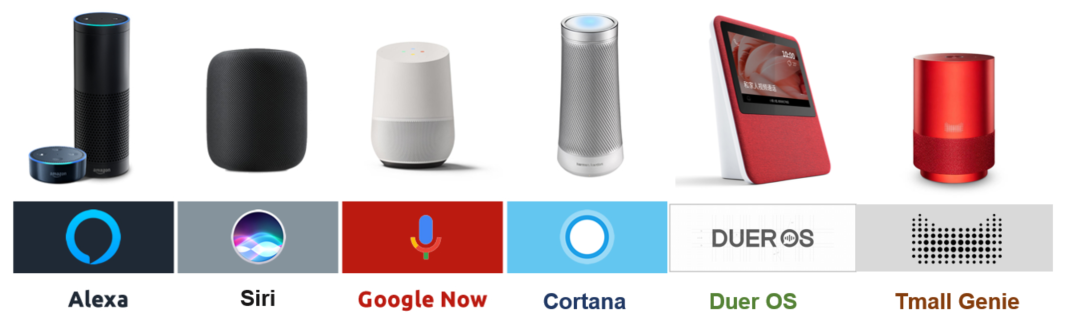
\includegraphics[width=0.9\linewidth]{Picture/Sprachassistenten}
	\caption[Sprachassistenten auf dem Markt\cite{homeAssistants}]{Sprachassistenten auf dem Markt\cite{homeAssistants}}
	\label{fig:sprachassistenten}
\end{figure}

Dabei gehen die Sprachassistenten unterschiedlich mit den Eingabedaten der Nutzer um. Aus den Datenschutzrichtlinien der Anbieter lassen sich keine exakten Informationen finden, was im Detail mit den Eingabedaten eines Nutzers geschieht. Im Folgenden werden die Datenschutzrichtlinien der einzelnen Anbieter kurz beschrieben.

Amazons Alexa verwendet alle Nutzereingaben, um den Sprachservice zu verbessern und personalisierte Werbung anzuzeigen. Eine Beschränkung der Datennutzung für verschiedene Bereiche ist möglich, wodurch sich allerdings auch die Funktionalität einschränkt \cite{alexaPrivacy}.

Google Assistant verwendet die gleichen Berechtigungen, welche für die mobile App des Anbieters gelten \cite{googleShare}. Eine abweichende Einstellung zur mobilen App ist dabei nicht möglich. Die Interaktion mit Google Assistant kann für die personalisierte Werbung genutzt werden, wie sonstige Suchanfragen \cite{googlePrivacy}.

Bei Siri müssen Dienste aktiviert sein, um darauf zurückgreifen zu können. Um die Aussprache und die Funktionalität zu verbessern, werden Daten wie Name, Kontakte, Musik, Suchaktivitäten und weitere Informationen verschlüsselt übertragen. Die Daten werden nicht mit der Apple ID genutzt, sondern mit zufällig erstellter Kennung. Dadurch wird die Privatsphäre für Nutzer gewährleistet \cite{siriPrivacy}.

In den Datenschutzeinstellungen von Microsofts Cortana wird darüber informiert, dass bestimmte Daten \glqq [...] wie z. B. ihre Suchen, Kalender, Kontakte und Orte. [...]\grqq{}\cite{cortanaAssistent} gespeichert werden. Die Datennutzung von Cortana als Personal Assistant ist konfigurierbar. Sind die personalisierten Informationen deaktiviert, kann Cortana nur für Anwendungen wie der Suche und das Festlegen eines Timers genutzt werden. Cortana verwendet personenbezogene Daten nicht für personalisierte Werbung. 

Baidu DuerOS sammelt ebenfalls Nutzerdaten, um die Sprachverarbeitung des Sprachassistenten zu verbessern. Qi Lu verweist auf die vielen Szenarien in denen Baidu Daten sammelt, womit Baidu der Sprung an die Weltspitze im Bereich Künstliche Intelligenz gelingen soll. Die persönlichen Daten eines Nutzers werden übermittelt. Dabei bietet Baidu keine konfigurierbare Privatsphäre an \cite{baiduAI}. 

Seit Februar 2018 gibt es den Sprachassistenten Mycroft Mark II, indem Offenheit und Privatsphäre vereint werden \cite{mycroftsmartspeaker}. Die Funktionalitäten sind hier begrenzt, da der Sprachassistent keine Daten speichert um den Benutzerkontext weiter zu trainieren und zu verstehen.
\section{Motivation}\label{sec:motivaiton}
Zu Beginn wurde durch eine Meinungsumfrage überprüft, ob bei Sprachassistenten mehr Datenschutz gewünscht ist. Dabei haben sich 110 Teilnehmer an der Umfrage beteiligt. Die Teilnehmer umfassten folgende Altersgruppen:
\begin{itemize}
	\item 1 bis 18 Jahre 
	\item 19 bis 25 Jahre
	\item 26 bis 35 Jahre
	\item 36 und älter	
\end{itemize}

55,5 \% der Teilnehmer waren männlich und 45,5\%  weiblich, wie in Abbildung \ref{fig:umfrage_teilnehmer} ersichtlich.

\begin{figure}[!h]
	\centering
	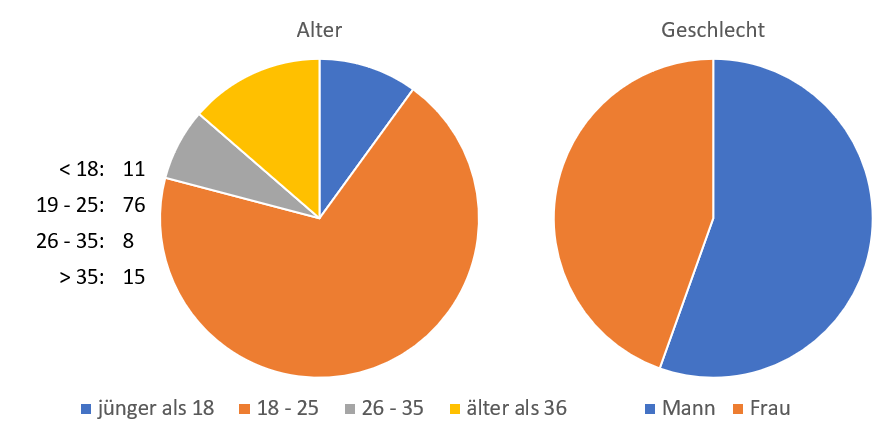
\includegraphics[width=0.9\linewidth]{Picture/umfrage_teilnehmer}
	\caption[Teilnehmer der Umfrage]{Teilnehmer der Umfrage}
	\label{fig:umfrage_teilnehmer}
	
\end{figure}

Den Teilnehmern wurden folgende Fragen gestellt:

\begin{enumerate}	
	\item Wie oft nutzen sie einen Sprachassistenten?
	\item Wissen sie was mit ihren Daten geschieht?
	\item Würden sie Geld für eine hohe Datensicherheit bezahlen?
	\item Wie viel Geld würden sie einmalig für eine hohe Datensicherheit einer Anwendung bezahlen?
	\item Bei welchen Anwendungen ist ihnen Privatsphäre besonders wichtig?	
\end{enumerate}

Bei der ersten Frage stellte sich heraus, dass 44,5\% einmal im Monat oder häufiger einen Sprachassistenten in Anspruch nehmen. In den USA wurde eine Studie von \glqq highervisibility\grqq{} durchgeführt, bei der mehr als 70\% der Teilnehmer einen Sprachassistenten mehr als einmal im Monat verwenden \cite{highervisibility}.
Ein direkter Vergleich der Umfrage mit der Studie aus der USA ist in Abbildung \ref{fig:umfrage_haeufigkeit} zu sehen.

\begin{figure}[!h]
	\centering
	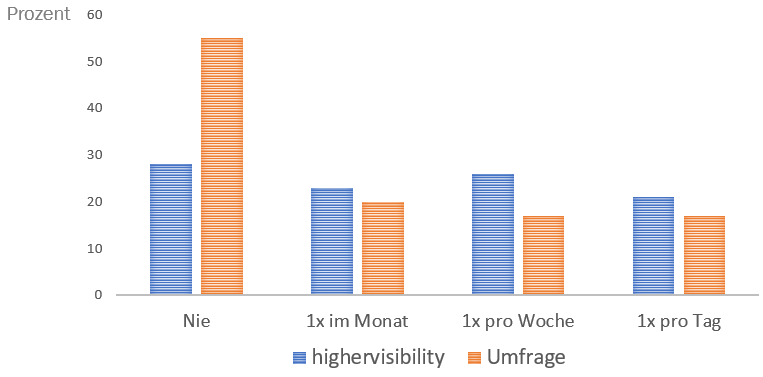
\includegraphics[width=0.9\linewidth]{Picture/umfrage_haeufigkeit}
	\caption[Nutzungshäufigkeit von Sprachassistenten]{Nutzungshäufigkeit von Sprachassistenten}
	\label{fig:umfrage_haeufigkeit}
\end{figure}

In der Studie wurden Menschen aus verschiedenen Altersgruppen und Herkunftsländern befragt. Die im Rahmen dieses Artikels durchgeführte Umfrage wurde überwiegend von jungen Leuten beantwortet.

\begin{figure}[!h]
 	\centering
 	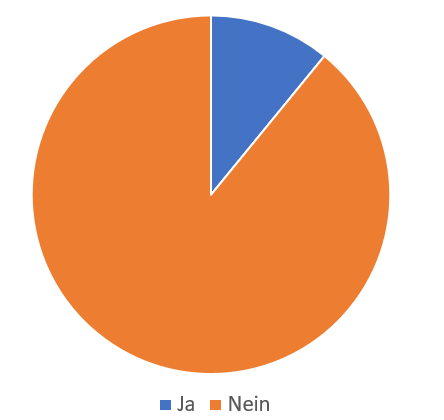
\includegraphics[width=0.5\linewidth]{Picture/umfrage_datenschutz}
 	\caption[Relevanz des Datenschutzes für die Umfrageteilnehmer]{Relevanz des Datenschutzes für die Umfrageteilnehmer}
 	\label{fig:umfrage_datenschutz}
\end{figure}

\newpage

Wie in Abbildung \ref{fig:umfrage_datenschutz} zu sehen ist, wissen 90\% der Teilnehmer nicht, was mit ihren Daten passiert. Die Zahlungsbereitschaft für Datensicherheit ist nach Altersgruppen in Abbildung \ref{fig:umfrage_geld_gruppen} visualisiert. Jeder Vierte würde für eine bessere Datensicherheit bezahlen und 56\% der Teilnehmer sind unsicher, ob sie dafür Geld ausgeben würden. Die Altersbetrachtung nach der Zahlungsbereitschaft ist bei der Gruppe unter 18 Jahren am geringsten. Die Schnittmenge der Teilnehmer, welche \glqq Ja\grqq{} oder \glqq Vielleicht\grqq{} angekreuzt haben, steigt mit zunehmendem Alter.

\begin{figure}[!h]
	\centering
	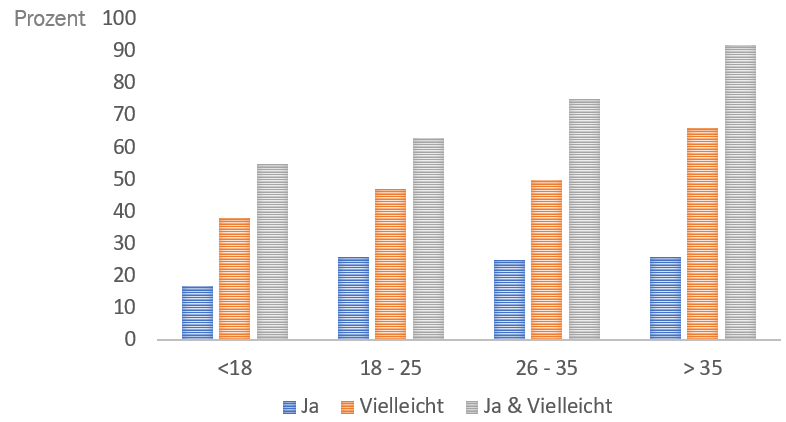
\includegraphics[width=0.9\linewidth]{Picture/umfrage_geld_gruppen}
	\caption[Zahlungsbereitschaft der Teilnehmer in verschiedenen Altersgruppen]{Zahlungsbereitschaft der Teilnehmer in verschiedenen Altersgruppen}
	\label{fig:umfrage_geld_gruppen}
\end{figure}

Der Betrag, welche die Teilnehmer für Anwendungen ausgeben würden variiert sehr und ist in Abbildung \ref{fig:umfrage_betrag} einzusehen. Ungefähr 15\% der befragten Teilnehmer sind nicht bereit dafür zu zahlen, während ein Großteil diese Bereitschaft hat.

\begin{figure}[!h]
	\centering
	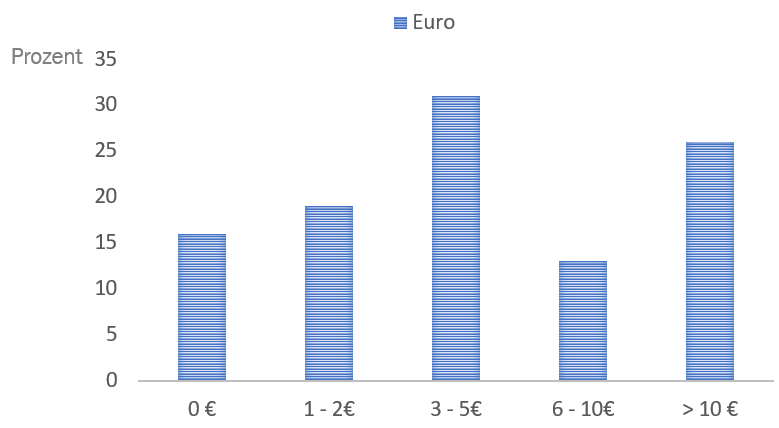
\includegraphics[width=0.9\linewidth]{Picture/umfrage_betrag}
	\caption[Zahlungsbereitschaft der Teilnehmer nach Betrag]{Zahlungsbereitschaft der Teilnehmer nach Betrag}
	\label{fig:umfrage_betrag}
\end{figure}

Wie Abbildung \ref{fig:umfrage_anwendung} zeigt, ist den Teilnehmern die Privatsphäre im Bereich Banking, Haussteuerung, Handysteuerung, Soziale Netzwerke und Chatting besonders wichtig.

Somit lassen sich folgende Schlussfolgerungen aus der Umfrage ziehen:
\begin{itemize}	
	\item Sprachassistenten werden in unterschiedlichem Umfang genutzt
	\item Die Nutzer wissen nicht, was mit ihren Daten geschieht
	\item Nutzer würden für den Schutz ihrer Daten bezahlen
	\item Datenschutz ist in den Bereichen Banking, Chatting, Haussteuerung, Social Media und Handysteuerung wichtig.
\end{itemize}

\begin{figure}[!h]
	\centering
	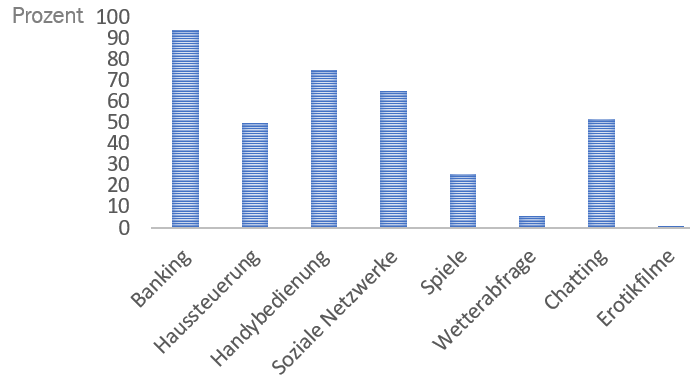
\includegraphics[width=0.9\linewidth]{Picture/umfrage_anwendung}
	\caption[Datenschutzrelevante Anwendungen der Umfrageteilnehmers]{Datenschutzrelevante Anwendungen der Umfrageteilnehmer}
	\label{fig:umfrage_anwendung}
\end{figure}

\section{Konzept}\label{sec:konzept}
Anhand der Umfrage wurde ein Konzept für einen Sprachassistenten entwickelt. Dabei wurden die Kosten für benötigte Ressourcen vernachlässigt. Eine wichtige Anforderung an das Konzept ist der Datenschutz. Die Entwurfsprinzipien für die mehrseitige Sicherheit von Daten nach Kai Rannenberg stellt folgende vier Punkte in den Vordergrund \cite{kairannenberg}:

\begin{enumerate}
	\item Datensparsamkeit
	\item Kontrollmöglichkeiten für den Nutzer 
	\item Auswahlmöglichkeiten und Verhandlungsspielräume 
	\item Dezentralisierung und Verteilung
\end{enumerate} 

Im Rahmen dieses Konzepts erfolgt die Fokussierung auf die ersten drei Punkte. Oftmals erfassen Anwendungen Daten eines Nutzers, die nicht der Verbesserung der Anwendungen dienen, sondern zur Analyse der Nutzer und dem Weiterverkauf verwendet werden. Deshalb soll durch das Konzept sichergestellt werden, dass eine Anwendung nur Daten von Nutzern bezieht, die diese auch tatsächlich benötigen. Des Weiteren sollen die erfassten Daten den Nutzern transparent dargestellt werden. Somit können Nutzer ihre erfassten Daten manipulieren bzw. anonymisieren. 

Daraus ergibt sich für den zu entwickelnden Sprachassistenten folgende Anforderungen:
\begin{itemize}
	\item Nutzergesteuerte Privatsphäre
	\item Funktionalität
	\item Performance
	\item Benutzerfreundlichkeit	
\end{itemize}

Durch die nutzergesteuerte Privatsphäre kann ein Nutzer bestimmen, welche Daten er von sich für bestimmte Anwendungen freigibt. Anwendungen benötigen jedoch zusätzliche Daten eines Nutzers, um dadurch Benutzerfreundlichkeit zu bieten. Ein Beispiel ist die Frage eines Sprachassistenten nach der Wettervorhersage. Weiß der Sprachassistent wo sich ein Nutzer aktuell befindet, so kann dieser die Wettervorhersage für die Position des Nutzer liefern. Sonst müsste der Sprachassistent zuerst den Nutzer fragen, für welchen Ort dieser eine Wettervorhersage wünscht. Will ein Nutzer seine Daten für eine Anwendung nicht freigeben, so kann er einen fiktiven Kontext festlegen. Damit kann der Nutzer diese Anwendung nutzen, jedoch auf Kosten der Benutzerfreundlichkeit.
\section{Architektur}\label{sec:architecure}

\captionsetup[table]{name=Abbildung}
\renewcommand\thetable{8}
\begin{table*}[!ht]
	\centering
	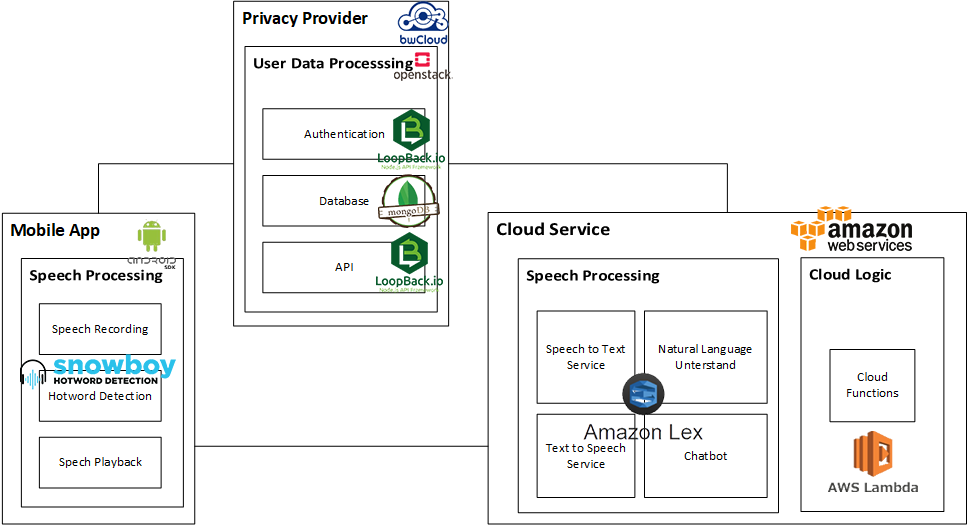
\includegraphics[width=1\linewidth]{Picture/Architektur}
	\caption[Archtiktur Übersicht]{Archtiktur Übersicht}
	\label{fig:architecure}
\end{table*}

Das im letzten Kapitel vorgestellte Konzept wird anhand der in Abbildung \ref{fig:architecure} aufgezeigten Architektur und Technologien umgesetzt. Dabei werden drei Komponenten zur Umsetzung benötigt:
 
\begin{itemize}
    \item Mobile App: Die Mobile App dient als Schnittstelle zum Nutzer. Der Nutzer kann über die App Spracheingaben tätigen sowie sein Profil und Privatsphäre konfigurieren.
    \item Cloud Services: Diese Komponente übernimmt die Sprachverarbeitung und die Erzeugung einer Ausgabe an den Nutzer. Dabei wird zur Erzeugung einer Antwort auf den Privacy Provider zugegriffen.
    \item Privacy Provider: Der Privacy Provider ist das Kernstück, wodurch dem Nutzer mehr Privatsphäre gewährleistet wird. Der genaue Aufbau sowie die Technologieauswahl wird im Folgenden beschrieben. 
\end{itemize}

Für die Kommunikation zwischen mobiler App und der Cloud Services mit dem Privacy Provider wurde eine RESTful \ac{api} ausgewählt. Die \ac{api} basiert auf der RESTful-Technologie, einem Architektur- und Kommunikationsmuster, das häufig bei der Entwicklung von Webdiensten zum Einsatz kommt. Mittels HTTP-Anforderungen wie z.B. GET, PUT-, POST- und DELETE- können Daten ausgetauscht und gespeichert werden \cite{restful-api}. Für die Umsetzung der „Speech Triggered Mobility Support and Privacy“ Anwendung, wurden virtuelle Maschinen, gehostet bei bwCloud, erstellt. Die bwCloud stellt mit Hilfe von OpenStack, \ac{iaas} für Forschung und Lehre in Baden-Württemberg bereit. Sie ermöglicht den Aufbau und Betrieb einer standortübergreifenden Infrastruktur zur Bereitstellung von Computer-Ressourcen \cite{bw-cloud}. Bei Bedarf kann eine bestehende virtuelle Maschine um zusätzliche Ressource erweitert werden, was die Skalierbarkeit des Projektes für zukünftige Anforderungen oder Erweiterungen vereinfacht. Die virtuelle Maschine wird mit Ubuntu Server 18.04.1 LTS betrieben. Mit Hilfe eines 2048Bit RSA Schlüssels kann Verbindung zur virtuellen Maschine hergestellt werden. Für die Umsetzung der REST \ac{api} wurden verschiedene Frameworks betrachtet. 

Loopback ist ein stark erweiterbares, Open-Source Node.js Framework, welches die Entwicklung schneller dynamischer End-to-End REST \ac{api}s ermöglicht. Loopback zeichnet sich durch eine große Community, ausgezeichnete Dokumentation, Vielzahl an Support Möglichkeiten (IBM, StrongLoop) sowie einem breitem Einsatzgebiet aus. Des Weiteren wird es unter anderem auch für kommerzielle Einsatzgebiete, wie z.B. bei der Bank of America, Symantec und der amerikanischen Energiebehörde (Department of Energy) eingesetzt \cite{loopback}.

Loopback ermöglicht es, REST \ac{api}s über ein Command Line Interface Wizard zu erstellen. Es können dynamische Modelle, basierend auf dem gewünschten Datenschema, erstellt werden. Ein weiterer ausschlaggebender Punkt für die Auswahl von Loopback, ist die Unterstützung von Beziehungen unter den erstellten Modellen und der automatischen Erstellung zugehöriger relationaler REST-Endpunkte. Das Framework ermöglicht die Umsetzung einfacher Authentifizierung und Autorisierung durch integrierte rollenbasierte Zugriffskontrollen. Eine Anmeldung von Drittanbietern und OAuth2 ist ebenfalls möglich \cite{mongodb}.

Für die Umsetzung wurde die Loopback Version 3.24.1 verwendet. Das Framework zeichnet sich durch seine Flexibilität aus. Es kann auf einem lokalen Server oder in der Cloud betrieben werden. Ein browserbasierter Explorer ermöglicht Interaktionen mit der \ac{api}. Loopback unterstützt die Anbindung von mehreren Datenspeichern. Für die Umsetzung wurde die Open Source Datenbank MongoDB ausgewählt. MongoDB ist ein verteiltes, flexibles, dokumentbasiertes Datenmodell. Daten werden in JSON-ähnlichen Dokumenten gespeichert. Dies ermöglicht eine Veränderung der Datenstruktur im Laufe der Zeit. Funktionen für Hochverfügbarkeit und Skalierung sowie geografische Verteilung sind einfach durchzuführen \cite{mongodb}. Diese Eigenschaften ermöglichen eine spätere Anpassung oder Verteilung der Infrastruktur.


\section{Prototyp}\label{sec:umsetzung}
In diesem Kapitel wird ein Prototyp vorgestellt, der die in dem vorherigen Kapitel aufgezeigte Architektur anhand eines Anwendungsbeispiels umsetzt. Im Folgenden wird das Anwendungsbeispiel beschrieben und anschließend die Umsetzung der einzelnen Komponenten der Architektur genauer erläutert.

\subsection{Anwendungsbeispiel}
Das Anwendungsbeispiel soll aufzeigen, wie durch einen Sprachassistenten die sprachbasierte Mobilitätsunterstützung gefördert und gleichzeitig ein feinkörniger Datenschutz für den Nutzer gewährleistet werden kann. Dabei werden durch das Anwendungsbeispiel folgende Funktionalitäten abgedeckt:

\begin{itemize}
    \item Ärzte in der Umgebung ermitteln.
    \item Einen Arzttermin aushandeln, wobei der Kalender eines Arztes mit dem Kalender des Nutzer abgeglichen wird.
    \item Optionale Mobilitätsunterstützung anfordern:
    \begin{itemize}
        \item Scala Mobile, Unterstützung des Nutzer beim Verlassen des Hauses. Kann notwendig sein, wenn der Nutzer beispielsweise nicht mehr alleine Treppen gehen kann.
        \item Abholservice, der den Nutzer zum Arzt und wieder nach Hause befördert.
    \end{itemize}
\end{itemize}

Ein Nutzer kann die Daten, die für diese Funktionalitäten notwendig sind, detailliert in einer mobilen App festlegen. Beispielsweise kann ein Nutzer seinen Standort automatisch via GPS ermitteln lassen, jedoch kann er diesen genauso in einem Textfeld eingeben. Der Nutzer kann seinen Kalender freigeben, jedoch sind für das Anwendungsbeispiel keine Termindetails notwendig. Es reicht aus zu wissen, ob ein Nutzer zu einem bestimmten Zeitpunkt verfügbar ist oder nicht. Aus diesem Grund kann ein Nutzer Termindetails, wie Titel und Beschreibung eines Termins ausblenden. Mehr Details zur Schützung der Privatsphäre werden im Laufe des Kapitel aufgezeigt. 
\subsection{Privacy Provider}

\setcounter{figure}{8}  
\begin{figure}[!ht]
	\centering
	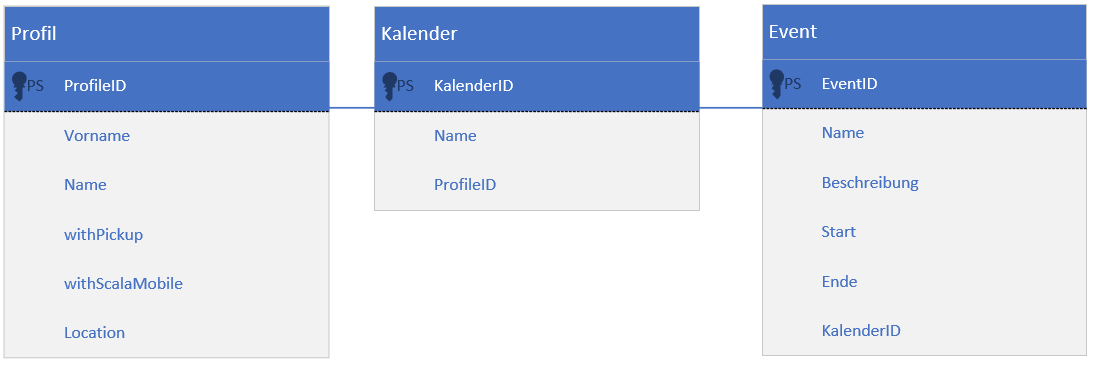
\includegraphics[width=1\linewidth]{Picture/Datenmodell}
	\caption[Datenmodell]{Datenmodell des Anwendungsfalls}
	\label{fig:datenmodell}
\end{figure}

In dem bereitgestellten Privacy Provider sollen Informationen zum Nutzerkontext gespeichert werden. Das Datenmodell ist speziell für die Anwendungsfälle beschrieben. Dabei werden personenbezogene Daten und freie Zeiten benötigt. Der Nutzerkontext wird durch dieses Datenmodell nur sehr eingeschränkt beschrieben. Allerdings kann das Datenmodell erweitert werden.

In diesem Datenmodell, welches in Abbildung \ref{fig:datenmodell} aufgezeigt ist, kann der Benutzer verschiedene Profile auswählen. So kann der richtige Name angegeben oder die Identität hinter einen anderen Namen verborgen werden. In dem Profil werden Angaben zur Mobilität hinterlegt, z.B. ob ein Fahr-Service und ein Scala Mobile benötigt wird. Mit den Profildaten sind die Kalender verknüpft. Die Daten werden direkt vom Smartphone ausgelesen, aber es können auch weitere Online-Kalender hinzugefügt werden. Schließlich beinhaltet ein Kalender mehrere Events. Für den Ort gibt es das Location-Feld. Die Location kann über den GPS-Sensor bestimmt oder es kann ein Ort eingegeben werden.

\subsection{Mobile App}
Die Mobile App dient einerseits als Interaktionsschnittstelle zwischen Nutzer und Sprachassistent und andererseits als Konfigurator der Privatsphäre. Die App bietet folgende vier Ansichten:

\begin{itemize}
    \item Registrierung: Ein neuer Nutzer kann sich mit seiner E-Mail und einem Passwort beim Sprachassistenten registrieren. Dabei kann der Nutzer zwischen den Profiltypen Privat, Arzt oder Mobilitätsunterstützung auswählen. Je nach Profiltyp werden unterschiedliche Privatsphäre-Einstellungen vorkonfiguriert. Standardmäßig ist ein privates Profil nur für den Besitzer zugänglich, wohingegen die Profiltypen Arzt und Mobilitätsunterstützung öffentlich zugänglich sind. 
    \item Login: Ein registrierter Nutzer kann sich mit seiner E-Mail und seinem Passwort bei dem Sprachassistenten anmelden.
    \item Sprachassistent: Der Sprachassistent ist die Hauptansicht der App, welche erscheint, sobald ein Nutzer eingeloggt ist. Gleichzeitig wird auch die Hotword Detection gestartet, welche mit Snowboy von Kitt.au realisiert wurde \cite{SnowboyHotwordDetection}. Die Hotword Detection lauscht lokal auf dem Smartphone, bis das Signalwort \glqq Butler\grqq{} erkannt wird, dabei werden keine Daten gespeichert und an Dritte weitergegeben. Nachdem Erkennen des Signalwortes wird die Sprachverarbeitung aufgrund besserer Performance in die Cloud verlagert. Sobald eine Interaktion zwischen Nutzer und Sprachassistent beendet ist, wird die Hotword Detection wieder aktiviert. Des Weiteren werden alle Ausgaben des Sprachassistenten auf der Ansicht ausgegeben. Die Audioaufnahme und Wiedergabe wurde mit der Android \acrshort{sdk} umgesetzt.
    \item Einstellungen: Diese Ansicht bietet dem Nutzer die Möglichkeit, sein Profil und Privatsphäre-Einstellungen zu konfigurieren. Für das Profil kann der Vor- und Nachname festgelegt werden. Der Standort kann entweder per Texteingabe oder per GPS ermittelt werden. Bei der Ermittlung des Standortes per GPS kann der Nutzer entscheiden, ob der Standort einmalig abgerufen wird oder die App automatisch diesen aktualisiert. Der Nutzer kann seinen Kalender der App zur Verfügung stellen. Dabei kann zusätzlich das automatische Aktualisieren des Kalenders oder das Verstecken von Details, wie Titel und Beschreibung eines Termins, aktiviert werden. Somit wird nur Zugriff auf die für den Anwendungsfall relevante Daten gewährleistet. Andere personenbezogene Daten, wie Name des Kalenders oder des Besitzers kann die App nicht ermitteln. Als Nächstes kann der Nutzer Mobilitätsunterstützungen festlegen, die beim Zustande kommen eines Termins mit einem Arzt standardmäßig angefordert werden. Dabei kann einerseits Scala Mobile, welches dem Nutzer beim Verlassen des Hauses hilft, oder anderseits ein Abholservice, der den Nutzer zum Arzt befördert, angefordert werden. Das Profil sowie die Privatsphäre-Einstellungen werden mit dem Privacy Provider synchronisiert. Durch diese App-Ansicht kann die im Konzept vorgestellte Datensparsamkeit  sowie die Nutzergesteuerte Privatsphäre ermöglicht werden.
\end{itemize}

\begin{figure}[!ht]
	\centering
	\begin{subfigure}[t]{0.48\linewidth}
		\centering
		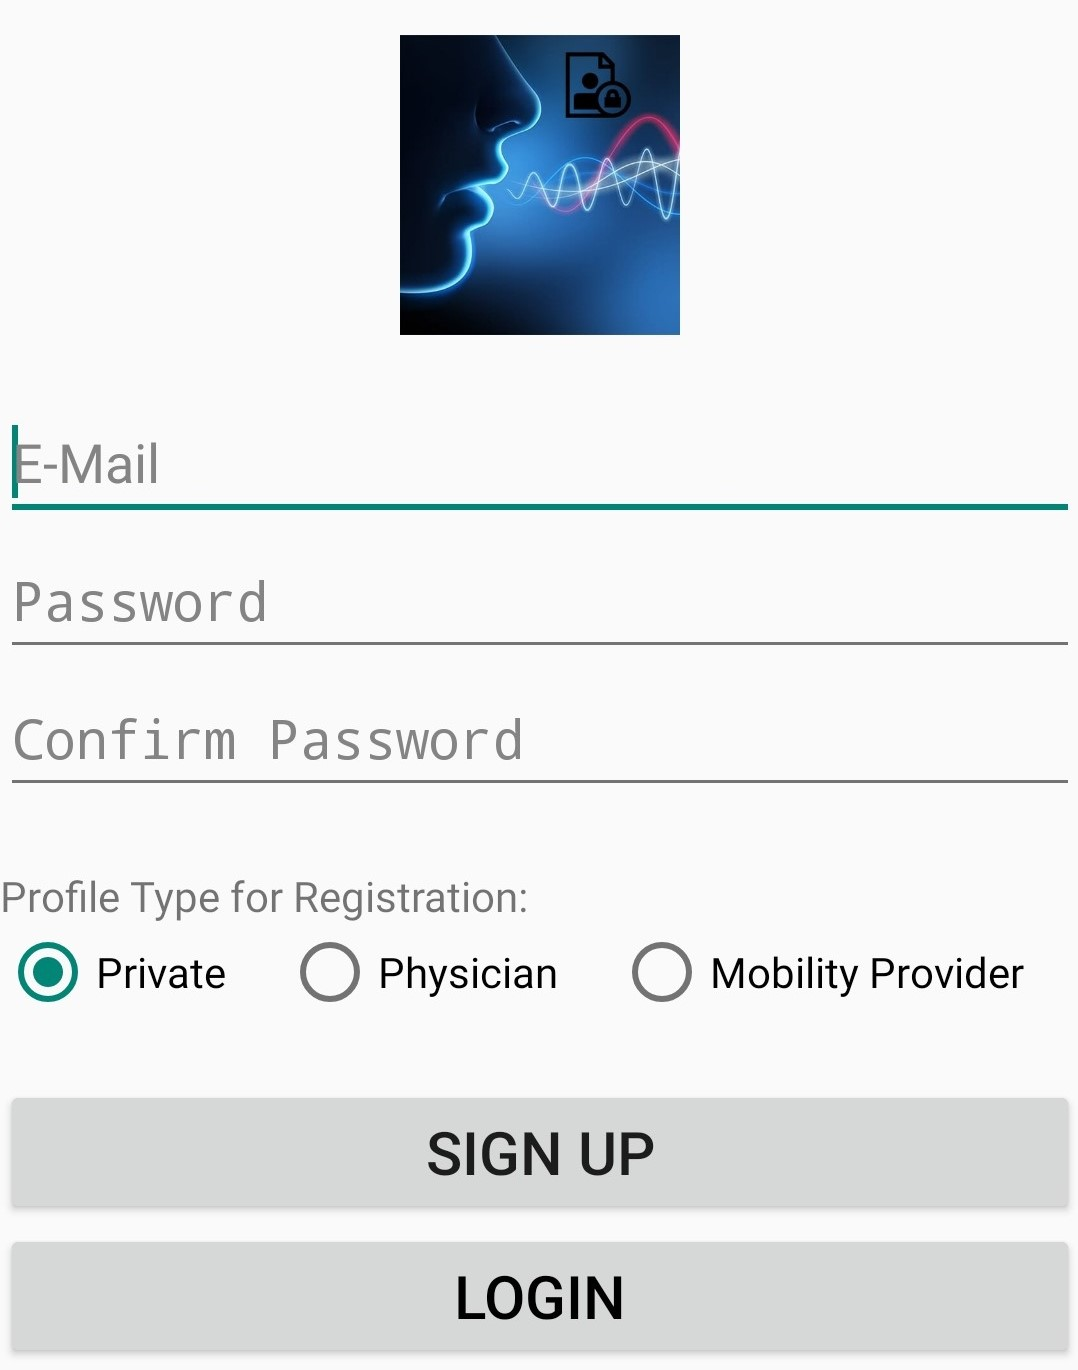
\includegraphics[width=1\linewidth]{Picture/MobileApp_Screenshot-2}
		\caption{Registrierungs-Ansicht}
		\label{fig:prototyp2}
	\end{subfigure}
	\bigskip 
	\begin{subfigure}[t]{0.48\linewidth}
		\centering
		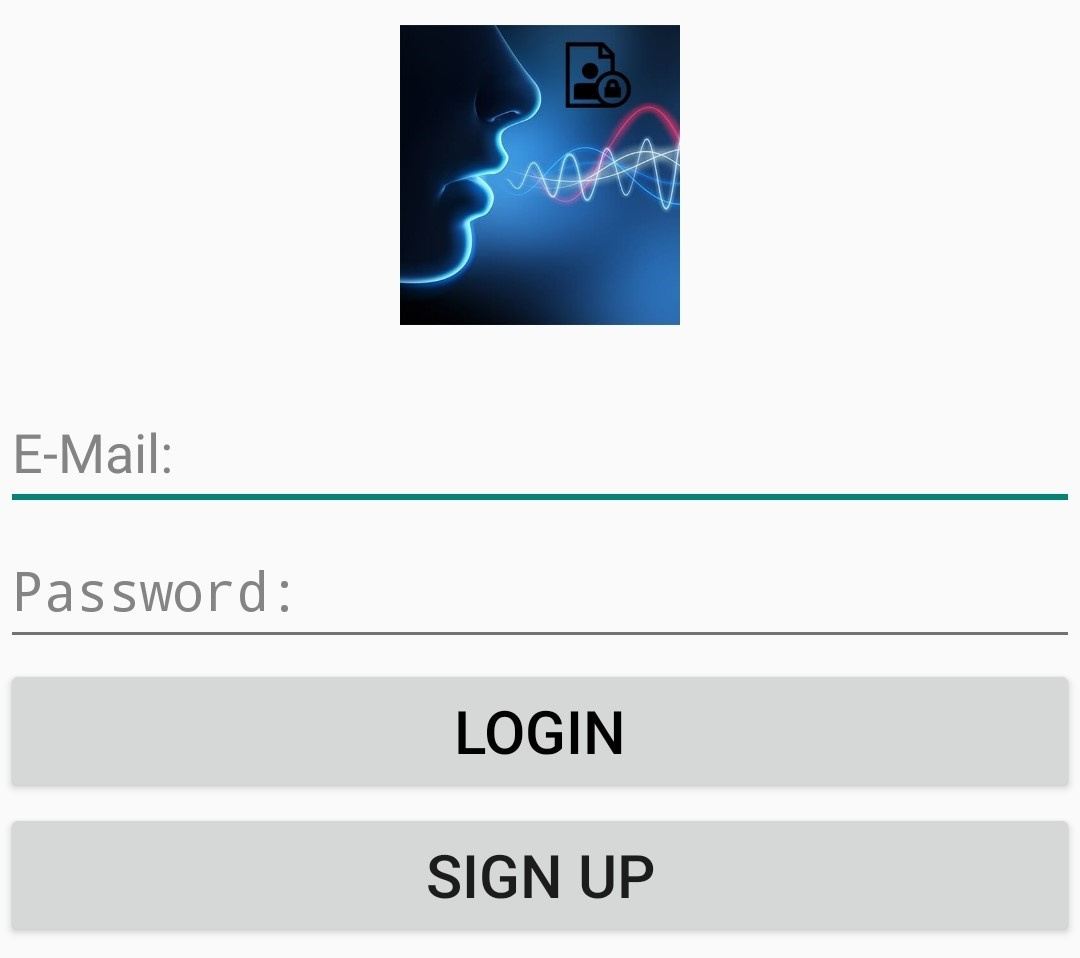
\includegraphics[width=1\linewidth]{Picture/MobileApp_Screenshot-1}
		\caption{Login-Ansicht}
		\label{fig:prototyp1}
	\end{subfigure}
	\bigskip 
	\begin{subfigure}[t]{0.48\linewidth}
		\centering
		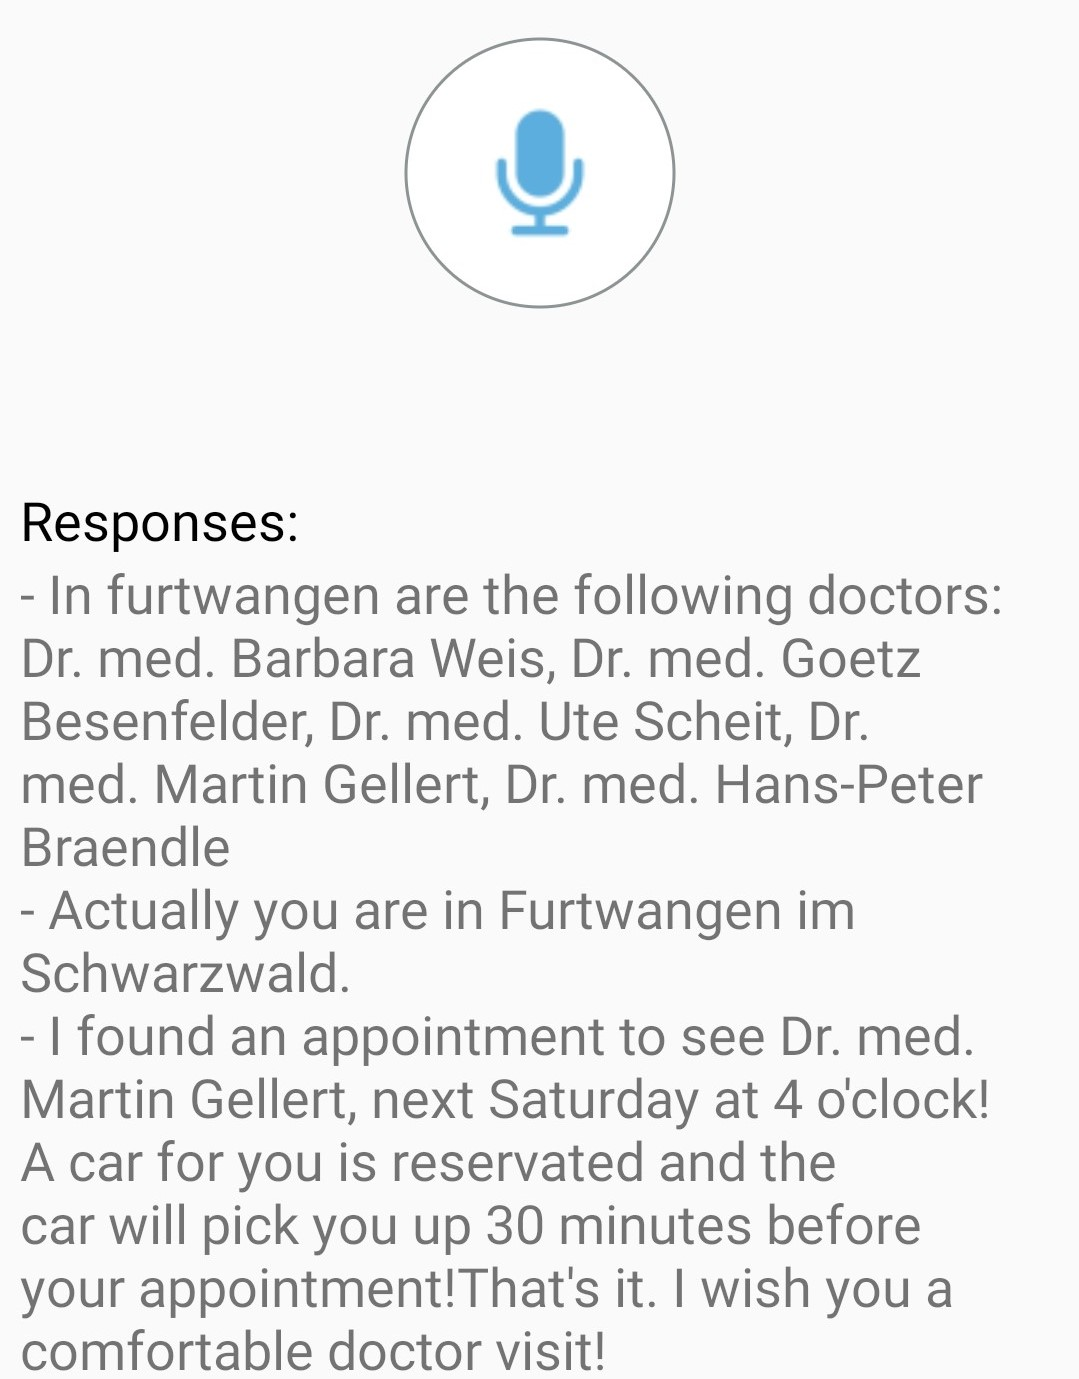
\includegraphics[width=1\linewidth]{Picture/MobileApp_Screenshot-3}
		\caption{Sprachassistent-Ansicht}
		\label{fig:prototyp3}
	\end{subfigure}
	\begin{subfigure}[t]{0.48\linewidth}
		\centering
		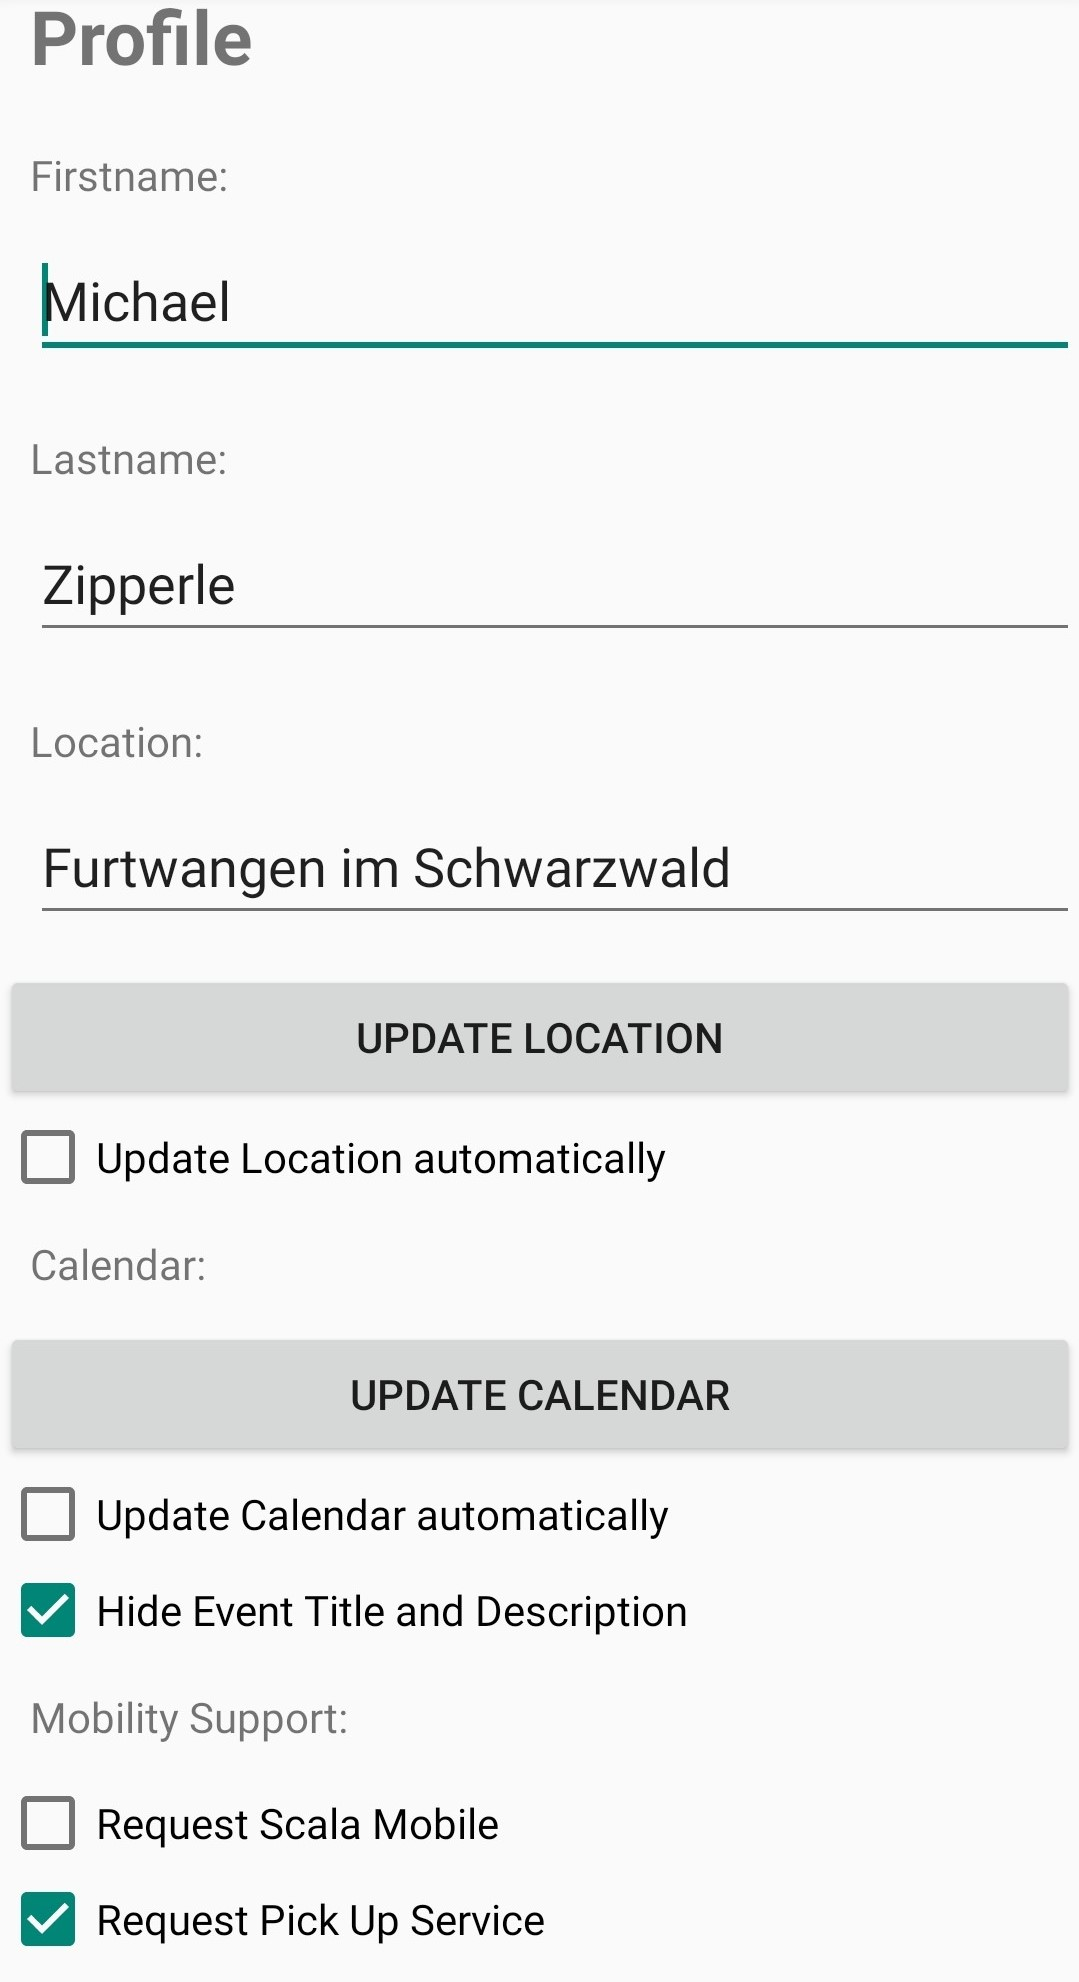
\includegraphics[width=1\linewidth]{Picture/MobileApp_Screenshot-4}
		\caption{Einstellungen-Ansicht}
		\label{fig:prototyp3}
	\end{subfigure}
	\caption{Mobile App}
	\label{fig:mobileapp}
\end{figure}
\subsection{Cloud Service}
Sobald das Signalwort \glqq Butler\grqq{} von der Hotword Detection erkannt wurde, wird die weitere Verarbeitung der Spracheingabe eines Nutzers in der Cloud durchgeführt. Zur Realisierung wurden folgende \ac{aws} eingesetzt:

\begin{itemize}
    \item Amazon Lex: Amazon Lex dient als Konversations-Schnittstelle für Sprache und Text. Durch fortschrittliches Deep Learning kann Sprache zu Text umgewandelt und die Textabsicht ermittelt werden. Anhand der Textabsicht kann eine Ausgabe erzeugt werden, welche anschließend von Text zu Sprache konvertiert wird \cite{AmazonLex}. Im Prototyp wird Amazon Lex für die o.g. Funktionalitäten eingesetzt. Zur Erzeugung einer Antwort auf eine Textabsicht wird eine Amazon Lambda Funktion gestartet.
    \item Amazon Lambda: Amazon Lambda bietet eine Plattform in der Cloud, auf der eine Anwendung bzw. Programmcode ausgeführt werden kann, ohne dass ein Server manuell bereitgestellt und verwaltet werden muss. Die Anwendung wird durch ein Event gestartet und nach der Beendigung dieser werden die Ressourcen wieder freigegeben. Amazon Lambda skaliert automatisch anhand der Anzahl an Events \cite{AmazonLambda}. Somit wurde auf Basis von Amazon Lambda eine Anwendung entwickelt, die anhand der Textabsicht des Nutzers, eine dynamische Antwort erzeugt. Durch den Access Token des Nutzers kann die Anwendung auf den Privacy Provider zugreifen, um die notwendigen Information zur Erzeugung der Antwort abzurufen. Somit konnte durch die Anwendungen die Aushandlungen eines freien Arzttermins zwischen Arzt und Nutzer realisiert werden.
\end{itemize}

Durch die Auslagerung der ressourcenintensiven Sprachverarbeitung in die Cloud kann dem Nutzer eine hohe Performance und Benutzerfreundlichkeit gewährleistet werden.
\subsection{Datenfreigabe}
Um Daten vom Privacy Provider nutzen zu können, ist zunächst eine Authentifizierung des Nutzers erforderlich. Hierzu werden die Anmeldedaten in der mobilen App eingegeben. Wird auf den Login-Button geklickt, wird der Nutzer durch den Privacy Provider authentifiziert. Bei diesem Vorgang werden dem Nutzer Lese-, Schreib-, und Ausführungsrechte gewährt, sodass Daten verändert und verschiedene Funktionen ausgeführt werden können. Außerdem wird ein zeitlich begrenzter Schlüssel erzeugt, mit dem der Nutzer Anwendungen Zugriff auf seine Daten gewähren kann. Welche Daten von einer Anwendung lesbar sind, kann der Nutzer in der mobilen App freigeben. Abbildung \ref{fig:accesstoken} zeigt beispielhaft eine Authentifizierung und anschließende Aktualisierung des Standortes des Nutzers mittels des Schlüssels.  

\begin{figure}[!ht]
	\centering
	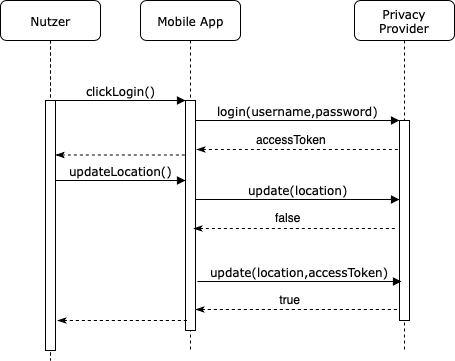
\includegraphics[width=1\linewidth]{Picture/AccessToken.png}
	\caption[Datenfreigabe im Privacy Provider]{Datenfreigabe im Privacy Provider}
	\label{fig:accesstoken}
\end{figure}





%\section{Zukünftige Arbeit}
Dieser Artikel zeigt das Problem aktueller Sprachassistenten auf. Mit dem vorgestelltem Konzept kann dem Nutzer eine bessere Privatsphäre gewährleistet werden. Im letzten Kapitel wurden einige Technologien zur Umsetzung dieses Konzeptes vorgestellt. Es zeigte sich, dass es eine große Auswahl an Technologien im Bereich der Sprachverarbeitung gibt. Als nächsten Schritt müssten diese Technologien evaluiert werden, um eine Technologieauswahl treffen zu können. Anhand dieser Auswahl kann festgelegt werden, welche Ressourcen die private Cloud zur Nutzung dieser Technologien benötigt. Des Weiteren lässt sich anhand der benötigten Ressourcen sowie Technologien ein Kostenmodell erstellen. Dieses kann genutzt werden, um eine erneute Umfrage bzw. Interviews mit möglichen Zielgruppen durchzuführen. Die Umfrage soll zeigen, ob die Zielgruppen bereit sind, zusätzliche Kosten für eine bessere Privatsphäre zu bezahlen. Danach kann mit einer prototypischen Entwicklung des Sprachassistenten begonnen werden. Zusätzlich gilt es ein Konzept zu entwickeln, mit welchem Apps auf unerwünschte Datenweitergabe an Dritte geprüft werden können. 
\section{Zusammenfassung}

Durch den entwickelten Prototyp, welcher dem Nutzer Datenschutz und Kontrollmöglichkeiten bietet, konnten einige Rückschlüsse gezogen werden. Dabei konnte die Konzeption bei der Implementierung berücksichtigt werden und Aspekte der mehrseitigen Sicherheit und benutzergesteuerten Privatsphäre finden sich ebenfalls im Prototyp. Der Prototyp besteht aus der Sprachverarbeitungsumgebung (Cloud Services), der Mobile App und dem Privacy Provider.

Anhand der genutzte Cloud Services von Amazon konnten die Funktionalitätsanforderungen erfüllt werden. Aktuell unterstützen die sprachbasierten Cloud Services von Amazon kein Deutsch, deshalb wurde der Prototyp mit Englisch als Sprache umgesetzt. Amazon kündigte jedoch an, bald mehr Sprachen, unter anderem auch Deutsch, anzubieten. Außerdem kann durch die erfüllten DSVGO-Richtlinien der Sprachservices der Datenschutz für die Nutzer gewährleistet werden. Durch die Verwendung der sprachbasierten Cloud Services müssen sich Entwickler nicht detailliert mit der Sprachverarbeitung auseinandersetzen, sondern können auf abstrakter Ebene eine Anwendung entwickeln.  
Bevor ein Nutzer den Sprachassistenten nutzen kann, muss dieser sich authentifizieren. Somit wird der Zugriff vor nichtberechtigten Personen geschützt. In der App können Nutzer verschiedene Profile mit unterschiedlichen Daten anlegen. Hierbei ist die Verwendung von Pseudoprofilen möglich. Im Hinblick auf das Konzept zur mehrschichtigen Sicherheit ist dies wichtig, um Auswahlmöglichkeiten und Verhandlungsspielräume für den Nutzer zu schaffen. Die Nutzerdaten sind in einem Privacy Provider abgelegt. Auch für den Privacy Provider gilt das Konzept der mehrseitigen Sicherheit. Hier ist die Dezentralisierung und Verteilung von großer Bedeutung. Durch die Technologie- und Anbieterauswahl wird auf allen Ebenen der Datenschutz berücksichtigt. Die Daten sind in Deutschland, womit auch eine Rechtslage angewendet wird, die deutlich strenger bei der Datenhaltung ist. Allerdings gibt es beim Privacy Provider auch noch Optimierungspotenzial. Zum einen soll der Ressourcenzugriff konfigurierbarer durch Berechtigung, Dauer und Filterung gestaltet werden. 

In diesem Prototyp wurden nur ein paar Anwendungsfälle umgesetzt. Je nach Nutzer variieren die Anforderungen an einen Sprachassistenten. Verschiedene Anwendungen sollten anhand der Bedürfnisse eines Nutzer aktiviert oder deaktiviert werden können. Dieses Funktionalität könnte den Prototyp in der Zukunft erweitern. Dabei müssen die angebotenen Anwendungen die Nutzer über verwendeten Daten informieren und damit Transparenz  schaffen. Um ein Ökosystem zu schaffen, indem jede Anwendung auf die Daten zugreifen kann, muss ein Standard über die Datenablage geschaffen werden. Andernfalls müssen die Anwendungen die Nutzerdaten selbst verwalten und das Konzept über die Trennung von Daten und Anwendung wäre hinfällig. 

In diesem Artikel wird an verschiedenen Stellen auf das Potenzial von Sprachassistenten verwiesen. Durch die angenehme Bedienung von der Systemintelligenz bietet es einen Mehrwert im Alltag. Allerdings müssen sich verschiedene Branchen öffnen und Schnittstellen anbieten, sodass Buchungen und Reservierungen nicht nur per E-Mail oder Telefon möglich sind. Ist die Infrastruktur von Unternehmen geschaffen, werden Sprachassistenten zusätzlich an Attraktivität für die Nutzer gewinnen.
\section{Danksagung}
Diese Artikel wurde im Rahmen eines Semesterprojekts an der Fachhochschule Furtwangen und unter Betreuung von Prof. Dr. Achim P. Karduck erstellt, dem wir für die gute Betreuung und die vielen Denkanstöße danken.
% *** END OF SECTIONS ***---------------------------------------------


% Can use something like this to put references on a page
% by themselves when using endfloat and the captionsoff option.
\ifCLASSOPTIONcaptionsoff
  \newpage
\fi

\printbibliography

\end{document}


